% This is samplepaper.tex, a sample chapter demonstrating the
% LLNCS macro package for Springer Computer Science proceedings;
% Version 2.20 of 2017/10/04
%
\documentclass[runningheads]{llncs}
%


% inlined bib file
\usepackage{filecontents}




%% Save the class definition of \subparagraph
\let\llncssubparagraph\subparagraph
%% Provide a definition to \subparagraph to keep titlesec happy
\let\subparagraph\paragraph
%% Load titlesec
%\usepackage[compact]{titlesec}
%% Revert \subparagraph to the llncs definition
\let\subparagraph\llncssubparagraph


%\usepackage{lipsum,mwe,cuted}
\usepackage{float}%%%%提供浮动体的[H]选项,进而取消浮动
\usepackage{caption}%%提供\captionof命令


\pagestyle{plain}


\usepackage{graphicx}
\usepackage{verbatim}
\usepackage{caption}
%

\usepackage[noend]{algpseudocode}


\usepackage{amsmath}
\usepackage{amssymb}
%\usepackage{amsthm}

\usepackage{graphicx}
%\usepackage{geometry}
%\usepackage{subfigure}
\usepackage{url}
\usepackage{multirow}
\usepackage{listings}
\usepackage{cite}
\usepackage{array}
\usepackage{enumerate}
\usepackage{booktabs}
\usepackage{color}
\usepackage{soul}
\usepackage{multicol}
%\usepackage{algcompatible}
%\usepackage[compatible]{algpseudocode}

%\usepackage[algo2e]{algorithm2e}
\usepackage{algorithm}
%\usepackage{algorithmic}
% Used for displaying a sample figure. If possible, figure files should
% be included in EPS format.
%
% If you use the hyperref package, please uncomment the following line
% to display URLs in blue roman font according to Springer's eBook style:
% \renewcommand\UrlFont{\color{blue}\rmfamily}






\makeatletter
\newenvironment{breakablealgorithm}
  {% \begin{breakablealgorithm}
   \begin{center}
     \refstepcounter{algorithm}% New algorithm
     \hrule height.8pt depth0pt \kern2pt% \@fs@pre for \@fs@ruled
     \renewcommand{\caption}[2][\relax]{% Make a new \caption
       {\raggedright\textbf{\ALG@name~\thealgorithm} ##2\par}%
       \ifx\relax##1\relax % #1 is \relax
         \addcontentsline{loa}{algorithm}{\protect\numberline{\thealgorithm}##2}%
       \else % #1 is not \relax
         \addcontentsline{loa}{algorithm}{\protect\numberline{\thealgorithm}##1}%
       \fi
       \kern2pt\hrule\kern2pt
     }
  }{% \end{breakablealgorithm}
     \kern2pt\hrule\relax% \@fs@post for \@fs@ruled
   \end{center}
  }
\makeatother


\algblockdefx{SWITCH}{ENDSWITCH}[1]{\textbf{switch} #1\ \textbf{do}}{\algorithmicend}
\algblockdefx{CASE}{ENDCASE}[1]{\textbf{case} #1\textbf{:}}{\algorithmicend}

\makeatletter
\ifthenelse{\equal{\ALG@noend}{t}}%
  {\algtext*{ENDCASE}}
  {}%
\makeatother

\makeatletter
\ifthenelse{\equal{\ALG@noend}{t}}%
  {\algtext*{ENDSWITCH}}
  {}%
\makeatother



\renewcommand{\algorithmicrequire}[1]{\textbf{Input:} #1}
\newcommand{\deflet}{\textbf{let}}
\newcommand{\mystate}[1]{\State \textbf{let} {{}#1}}
\newcommand{\mystop}[1]{\State \textbf{stop} \myss{\myangle{{{}#1}}, s'}}
\newcommand{\myss}[1]{${{}#1}$}
\newcommand{\myangle}[1]{\langle {{}#1} \rangle}
\newcommand{\myif}[1]{\If{\myss{{{}#1}}}}
\newcommand{\myelse}[1]{\ElsIf{\myss{{{}#1}}}}

\begin{comment}
\newcommand{\SWITCH}[1]{\State \textbf{switch} #1\ \textbf{do} \begin{ALC@g}}
\newcommand{\ENDSWITCH}{\end{ALC@g}\State \textbf{end switch}}
\newcommand{\CASE}[1]{\State \textbf{case} #1\textbf{:} \begin{ALC@g}}
\newcommand{\ENDCASE}{\end{ALC@g}}
\newcommand{\CASELINE}[1]{\State \textbf{case} #1\textbf{:} }
\newcommand{\DEFAULT}{\State \textbf{default:} \begin{ALC@g}}
\newcommand{\ENDDEFAULT}{\end{ALC@g}}
\newcommand{\DEFAULTLINE}[1]{\State \textbf{default:} }
\end{comment}






\begin{document}
%
\title{Enhancing the User Privacy of SSO by Integrating PPID and SGX
}%\thanks{Supported by organization x.}}
%
%\titlerunning{Abbreviated paper title}
% If the paper title is too long for the running head, you can set
% an abbreviated paper title here
%
\author{}
\institute{}
\begin{comment}
\author{First Author\inst{1}\orcidID{0000-1111-2222-3333} \and
Second Author\inst{2,3}\orcidID{1111-2222-3333-4444} \and
Third Author\inst{3}\orcidID{2222--3333-4444-5555}}
%
\authorrunning{F. Author et al.}
% First names are abbreviated in the running head.
% If there are more than two authors, 'et al.' is used.
%
\institute{Princeton University, Princeton NJ 08544, USA \and
Springer Heidelberg, Tiergartenstr. 17, 69121 Heidelberg, Germany
\email{lncs@springer.com}\\
\url{http://www.springer.com/gp/computer-science/lncs} \and
ABC Institute, Rupert-Karls-University Heidelberg, Heidelberg, Germany\\
\email{\{abc,lncs\}@uni-heidelberg.de}}
\end{comment}
%
\maketitle              % typeset the header of the contribution
%
\begin{abstract}
Single sign-on (SSO) services are widely deployed in the Internet as the identity management and authentication infrastructure. After authenticated by the identity providers (IdPs), a user is allowed to log in to relying parties (RPs) by submitting an \emph{identity proof}(i.e., id token of OpenID Connect or SAML assertion).
However, SSO introduces the potential leakage of user privacy, indicated by NIST.  That is (\emph{a}) a curious IdP could track a user's all visits to any RP and (\emph{b}) collusive RPs could link the user's identities across different RPs, to learn the user's activity profile.
NIST suggests that the Pairwise Pseudonymous Identifier (PPID) should be adopted to prevent collusive RPs from linking the same user. PPID mechanism enables an IdP to provide a user multiple individual IDs for different RPs. Popular SSO protocols, such as OpenID Connect and SAML, have already provided PPID as the optional configuration. It is suggested by many identity service providers, such as NORDIC APIS and CURITY, PPID should be adopted in all SSO systems. However, PPID mechanism cannot protect user from IdP's tracking, as the generation of PPID requires the participation of RP ID .

In this paper, we propose an SSO system, Enhancing the User Privacy of SSO by Integrating PPID and SGX, named UP-SSO. UP-SSO provides the enhanced PPID mechanism to protect a user's activity profile of RP visits from both the curious IdP and the collusive RPs. 
It separates a IdP service into two parts, the server-side service and user-side service. The generation of PPID is shifted from IdP server to user client, so that IdP server no longer needs to learn RP ID. 
%Moreover, the user client is protected by Intel SGX. %Therefore, it would verify RP ID, generate PPID and transmit it to IdP server honestly. 
User client also transforms RP ID into one-time encrypted ID, used by IdP for identity token generation, instead of RP's real ID. The correctness of client can be verified by IdP through remote attestation.
The server-side service running on the IdP server still takes the responsibility of authenticating users, storing the private key, issuing the identity token and etc. 
The detailed design of UP-SSO is described in this paper, and the systemically analysis is provided to guarantee its security. 
We implemented the prototype system of UP-SSO, and the evaluation of prototype system shows the overhead is modest.

\keywords{SSO  \and Privacy \and Intel SGX.}
\end{abstract}
%
%
%


\section{Introduction}
\label{sec:intro}
Single sign-on (SSO) systems, such as OAuth, OpenID Connect (OIDC) and SAML, have been widely deployed for web authentication.
%nowadays as a convenient web authentication mechanism. 
SSO delegates user authentication on websites from online services (Relying Party, RP) to a third party (Identity Provider, IdP).
%, via a single authentication process. 
Using SSO, a user no longer needs to maintain multiple credentials for different RPs.
%, instead, she only maintains the credential for the IdP, which further provides identity proofs to RPs.
%For RPs, SSO shifts the burden of user authentication to IdPs and therefore reduces their security risks and costs. As a result, SSO has been widely integrated with modern web systems.
According to Alexa, the popular web traffic analysis site, 80 websites among the top-100 websites integrate SSO services~\cite{Alexa}.
%Meanwhile, many email and social networking providers such as Google, Facebook, Twitter, etc. have been actively serving as social identity providers to support social login.

However, the wide adoption of SSO also raises new privacy concerns. 
%Currently, more and more companies are interested in the users' online trace for business practices, such as accurate delivery advertising. For example, large internet service providers, such as Google, are interested in collecting users' online behavioral information for various purposes (e.g., Screenwise Meter~\cite{googlenews}). Now, by simply serving the IdP role, these companies can easily collect a large amount of data to reconstruct users' online traces. 
NIST~\cite{NIST2017draft} indicates that curious IdP or multiple collusive RPs could break the users' privacy in such ways. (1) \textbf{IdP-based login tracing}. The IdP knows the identities of the RP and user in each single login instance; (2) \textbf{RP-based identity linkage}. The RP learns a user's identity from the identity proof, so that malicious RPs could collude to link the user's login activities.
\begin{comment}
\item {\em IdP-based login tracing}. The IdP knows the identities of the RP and user in each single login instance.
%, to generate the identity proof.
%As a result, a curious IdP could discover all the RPs that the victim user attempts to visit and profile her online activities.
\item {\em RP-based identity linkage}. The RP learns a user's identity from the identity proof, so that malicious RPs could collude to link the user's login activities.
%When the IdP generates identity proofs for a user, while the same user identifier is used in identity proofs generated for different RPs, malicious RPs could collude to not only link the user's login activities at different RPs for online tracking but also associate her attributes across multiple RPs.
\end{comment}

%The IdP-based login tracing and RP-based identity linkage would bring the real threat to users. Imagine that, a user concerning her privacy would avoid leaving her full sensitive information at an application. She only leaves parts of her sensitive messages at each application, for example, using the real name on a social website and address on shopping website. And she would try not to leave any linkable message to avoid applications combining her information, such as email.
%However, the privacy leaks in SSO systems make her effort in vain. As long as a user employs the SSO system, such as Google Account, to log in to these applications, the applications providers and Google can combine her information based on the SSO account.


To protect user privacy, the Pairwise Pseudonymous Identifier (PPID) is suggested by NIST~\cite{NIST2017draft}, OIDC~\cite{OpenIDConnect} and SAML~\cite{SAMLIdentifier}.
%and popular SSO protocols, such as OpenID Connect (OIDC)~\cite{OpenIDConnect} and SAML~\cite{SAMLIdentifier}. 
That is, IdP should offer a user multiple individual IDs for different RPs. 
Thus, an RP cannot  correlate the  PPID  with user's PPID at another RP. 
%Thus, collusive RPs cannot link a user's logins targeting different RPs. 
More and more IdPs have adopted PPID to protect user privacy, such as Active Directory Federation Services and Oracle Access Management.
%~\cite{MS, Oracle}. 
And NORDIC APIS and CURITY also suggest adopting PPID in SSO to protect user privacy.
%~\cite{Nordic, Curity}.

Although PPID mechanism can protect user from RP-based identity linkage, the IdP-based identity linkage is not well prevented in SSO systems.
There have been many works on protecting user privacy in SSO systems, however, to the best of our knowledge, none of the existing techniques~\cite{SPRESSO, BrowserID, ZhangKSZR21, IsaakidisHD16} can offer the comprehensive protection of privacy or achieve it by integrating PPID. 
%Beside of PPID mechanism, there have been many works on protecting user privacy in SSO systems. 
Here we give a brief introduction of existing solutions
% for privacy-preserving SSO 
and explain the flaws of these schemes. 
\begin{itemize}
\item {\noindent\textbf{Simply hiding RP ID from IdP. }}For example, SPRESSO~\cite{SPRESSO} were proposed to defend against IdP-based login tracing by hiding RP ID from IdP. It uses the encrypted RP ID instead, and IdP issues the identity proof for this one-time encrypted ID. 
However, PPID is not available in this type of solution, as IdP cannot offer an RP a constant PPID with one-time irrelevant RP ID.
\item {\noindent\textbf{Proving user identity based on zero-knowledge proof. }}In this type of solution, such as EL PASSO~\cite{ZhangKSZR21}, the user needs to keep a secret $s$ and requires IdP to generate an identity proof for blinded $s$. Then user has to prove that she is the owner of $s$ without exposing $s$ to RP. 
However, whenever a user tries to visit RP at a new device, she must import  $s$ into this device. Thus, it is not convenient for user's login on multiple devices. 
%However, it is not convenient for user's login on multiple devices. For security consideration, the $s$ must be too long for user to remember.  And the user's identity is associated with the private $s$, therefore, if the user wants to log in to the RP on a new device, she must import the large $s$ into this device. 
%\item {\em Completely anonymous SSO system. }Anonymous SSO scheme is proposed to hide the user's identity to both the IdP and RPs in many manners. For example, the anonymous SSO~\cite{HanCSTW18} allows a user to visit the RP without exposing her identity to both IdP and RP based on zero-knowledge proof. However, it can only be applied to the anonymous services that do not identify the user, but not available in current personalized internet service.
\end{itemize}


%As discussed above, none of the existing SSO systems defend against both IdP-based login tracing and RP-based identity linkage, and provide the convenient SSO service on multiple devices at the same time.
%We remark that the problems cannot be solved, such as simply combining existing solutions together. The challenge is that, there is not a simple way for IdP to provide PPID without knowing the RP's identity.

In this paper, we propose UP-SSO, 
%Enhancing the User Privacy of SSO by Integrating PPID and SGX, 
the comprehensive protection against both IdP-based login tracing and RP-based identity linkage.
The key idea of UP-SSO is shifting PPID generation from server to user client,
so that IdP server can issue the identity proof containing user's PPID (denoted as $PPID_U$), by only requiring an one-time transformed RP ID (e.g., encrypted RP ID, denoted as $PPID_{RP}$). 
In UP-SSO system, the user client takes the responsibility for generating $PPID_U$ and transforming RP ID into $PPID_{RP}$,
%(as an identity proof must contain the RP ID to avoid misuse of token~\cite{YangLCZ18, WangZLG16, MainkaMS16, MainkaMSW17}). 
%For IdP, 
%it can only obtain an encrypted one-time RP ID, 
so that the IdP-based login tracing is not impossible as IdP no longer receives plain RP ID.
To be noticed is that the user-side service must be deployed at the user-controlled and IdP trusted environment, i.e., Intel SGX. 
With SGX, the secure hardware supported by intel CPU, the user-side service can be deployed at user's PC, and its integrity is guaranteed by \emph{Remote Attestation}, the mechanism provided by SGX.
%Moreover, other essential IdP services, such as user authentication and identity proof issuing,  must be deployed at server side for security consideration. 

%The overview of UP-SSO is shown in Figure~\ref{}. At the very beginning, user starts the visit to an RP (step 1). Then RP redirects user to IdP and the user is authenticated by IdP (step 2). After that, user invokes the user client (application protected by SGX) for PPID generation. To be noticed is that remote attestation must be conducted while the user client launches. After remote attestation, the user client and server are considered built a trust channel through a exchanged symmetric key. User client next retrieves the user ID (i.e., UID) from IdP server and RP (step 3). Then it generates the encrypted RP ID and PPID and sends them to IdP server to generate identity token (step 5). Following IdP issues the token with encrypted IDs and return it back to user ().   

%There have already been efforts on implementing authentication with security hardware, such as FIDO~\cite{fidouaf} UAF mode. It enables secure hardware (e.g., a smartphone) to store user's private key while the RP server stores the public key. Therefore, a user can be authenticated by the RP through a signed login challenge. However, compared with UP-SSO (as well as traditional SSO), FIDO does not provide an authority center, such as IdP. It brings about the problem that, the FIDO service cannot set accessibility limits without additional user information. For example, an RP requires that all the visitors must be adults. 
%In UP-SSO, the user only needs to be verified at IdP and the result can be included in an identity token. However, in FIDO system, the verification is not available except that user uploads specific information, which would link the user's accounts in different RPs. 

%To guarantee the security of UP-SSO, we provide the description of threat model and detailed systemic analysis, that shows UP-SSO prevents all the known attackers. Moreover, we have implemented a prototype of UP-SSO, including the servers, user client and user-side JavaScript codes. And we compare the performance of the UP-SSO prototype with a state-of-the-art SSO system (e.g., OpenID Connect). The time cost of UP-SSO and OpenID Connect is, respectively, about 154 and 113 ms. The overhead is modest.


\begin{comment}
We summarize our contributions as follows.
%我们的贡献
%提出协议
%考虑能否根据模型进行分析
%实现原型系统
%The main contributions of UPPRESSO are as follows:
\begin{itemize}
\item We propose the comprehensive solution to hide the users' login traces from both the curious IdP and malicious collusive RPs for convenient SSO system.
\item We formally analyze the security of XXX and show that it guarantees the security, while the users' login traces are well protected.
\item We have implemented a prototype of XXX, and compare the performance of the UP-SSO prototype with the state-of-the-art SSO systems (e.g., OIDC), and demonstrate its efficiency.
\end{itemize}
\end{comment}

\vspace{1mm}\noindent\textbf{Our contribution. }The main contribution of UP-SSO is that, it provides the PPID-included (containing $PPID_{RP}$ and $PPID_U$ ) identity proof without exposing RP ID to IdP, by shifting the $PPID_U$ generation from IdP server to user controlled device, and protecting it with the Intel SGX.
%we shift the PPID generation from IdP server to user controlled device, and protect it with the Intel SGX. It enables the IdP to provide the PPID-included identity token without exposing RP ID to IdP, while the user-side service is verified by IdP through remote attestation to guarantee its integrity.  
Therefore, UP-SSO offers the comprehensive solution to hide the users' login traces from both the curious IdP and malicious collusive RPs. 
%Moreover, it provides a new way of using secure hardware (i.e., Intel SGX) for SSO systems.

%文章结构
The rest of the paper is organized as follows. We first introduce the background in Section~\ref{sec:background}. Then, we describe the threat model, and our UP-SSO design in Sections~\ref{sec:threatmodel} and \ref{sec:design}, followed by a systemic analysis of security and privacy in Section~\ref{sec:analysis}. We provide the implementation specifics and experiment evaluation in Section~\ref{sec:implementation},  discuss the related work in Section~\ref{sec:relatedwork}, and conclude our work in Section~\ref{sec:conclusion}.

\section{Background}
\label{sec:background}
UP-SSO is compatible with OIDC, and achieves privacy protection based on the SGX.
Here, we provide a brief introduction on OIDC and the SGX.
\subsection{OpenID Connect and PPID}
OIDC~\cite{OpenIDConnect} is an extension of OAuth 2.0 to support user authentication, and has become one of the most prominent SSO authentication protocols. 
%Same as other SSO protocols~\cite{SAMLIdentifier}, OIDC involves three entities, i.e., {\em users}, the {\em identity provider (IdP)}, and {\em relying parties (RPs)}.
%PPID is suggested in OpenID Connect protocol to protect the user from a possible correlation among RPs.

\vspace{1mm}\noindent\textbf{Implicit flow of user login.}
OIDC supports three processes for the SSO authentication session, known as {\em implicit flow}, {\em authorization code flow} and {\em hybrid flow} (i.e., a mix-up of the previous two). Here, we choose the OIDC implicit flow as the example to illustrate the protocol. 
%In the implicit flow, an {\em id token} is generated as the identity proof, which contains a user identifier, an RP identifier, IdP's identifier, the validity period, and other requested attributes.
%The IdP signs the id token using its private key to ensure integrity.

\begin{figure}[t]
  \centering
  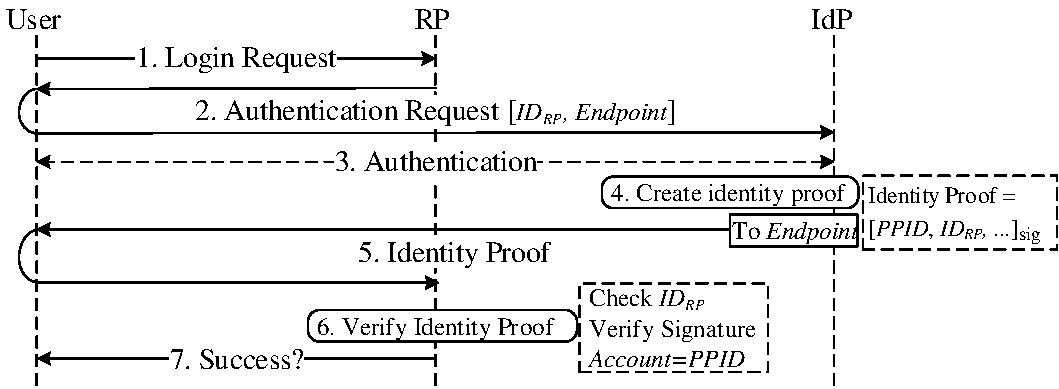
\includegraphics[width=\linewidth]{fig/OIDC1.pdf}
  \vspace{-5mm}
  \caption{The implicit protocol flow of OIDC.}
  \label{fig:OpenID}
  \vspace{-6mm}
\end{figure}

As shown in Figure~\ref{fig:OpenID}, 
At the beginning, user attempts to log in to an RP (step 1). Then RP constructs a request for identity proof, which is redirected by the user to the corresponding IdP. The request contains $ID_{RP}$, RP's endpoint other attributes (step 2). If the user has not been authenticated yet, the IdP performs an authentication process (step 3). Following, IdP signs the $ID_{RP}$ and PPID as the identity proof (step 4), and sends it back to the RP (step 5). Finally, the RP verifies the id token, extracts user identifier (step 6), and returns the authentication result to the user (step 7).
\begin{comment}
\item[1] At the beginning, user attempts to log in to an RP.
\item[2] RP constructs a request for identity proof, which is redirected by the user to the corresponding IdP. The request contains $ID_{RP}$, RP's endpoint other attributes.
\item[3] If the user has not been authenticated yet, the IdP performs an authentication process.
\item[4] IdP signs the $ID_{RP}$ and PPID as the identity proof.%If the RP's endpoint in the request matches the one registered at the IdP, it generates an identity token. Otherwise, IdP generates a warning to notify the user about potential identity proof leakage.
\item[5] IdP sends the identity proof back to the RP.
\item[6] The RP verifies the id token, and extracts user identifier.
\item[7] Finally, RP returns the authentication result to the user.
\end{comment}

\vspace{1mm}\noindent\textbf{Pairwise Pseudonymous Identifier (PPID).} 
PPID is the user identifier provided by IdP identifying a user. Different from the normal user ID, PPID is an RP-specific user ID. That is, while a user visits different RPs, IdP would provide different but constant user IDs (i.e., PPID) for these RPs.    
NIST~\cite{NIST2017draft} suggests that PPID should be either generated randomly and assigned to users by the IdP, or derived from other user's information if the derivation is done in an irreversible, unguessable manner. 
%that PPID should be used to prevent the user's account at the IdP from being easily linked at multiple RPs through use of a common identifier. 
%It also suggests that PPID should be either generated randomly and assigned to users by the IdP, or derived from other user's information if the derivation is done in an irreversible, unguessable manner (e.g., using a keyed hash function with a secret key). 
%For example, we have learned that, MITREid Connect, a popular open-source OIDC project, generates PPID using a secure random number generator, and stores the key-value map of corresponding RP and PPID.


\subsection{Intel SGX}
Intel Software Guard Extensions (Intel SGX)~\cite{costan2016intel} is the hardware-based security  mechanism provided by Intel processors.  Enclaves~\cite{costan2016intel} and remote attestation~\cite{costan2016intel} mechanism are offered by Intel SGX.
%It offers memory encryption that isolates specific application code and data in memory.
%It allows user-level code to allocate private regions of memory, called enclaves~\cite{costan2016intel}, which guarantees the running codes are well protected from the adversary outside the enclave.
 
\vspace{1mm}\noindent\textbf{Enclave.}
The enclave’s code and data is stored in Processor Reserved Memory (PRM). 
PRM cannot be directly accessed by other software, including system software and System Management Module code (Ring 2).
The Direct Memory Access (DMA) of PRM is also unavailable, as enclave is protected from other peripherals. That is, while the application is running inside the enclave, even the device owner cannot break its security, such as accessing or tempering the application's data.



\vspace{1mm}\noindent\textbf{Remote Attestation.} 
Remote attestation enables the software inside an  enclave to attest to a remote entity that it is trusted. 
%That is, during the attestation, the remote entity would receive an SGX attestation signature, containing the enclave’s measurement (a measurement of the code and data loaded in enclave).
The SGX remote attestation allows a player to verify the application's identity, intactness (never tampered), and that it is running securely within an enclave.
Moreover, with the remote attestation, the secure key exchange between the player and remote enclave application is also available.% even the application runs in a malicious environment.

 
\section{Threat Model}
\label{sec:threatmodel}
%UP-SSO is compatible with OIDC, consisted of a number of RPs, user agents(including browser and enclave application) and an IdP.
In this section, we describe the threat model and assumptions of the entities in UP-SSO.

\vspace{1mm}\noindent\textbf{Adversary Goal:} (1) The adversaries attempt to impersonate a user to log into an RP (\textbf{breaking the  security of SSO}); (2) the adversaries want to track a user's login trace (\textbf{breaking the privacy}).
\begin{comment}
\item \noindent\textbf{Breaking the security. }The adversaries can impersonate an honest user to log in to the honest RP.
\item \noindent\textbf{Breaking the privacy. }The adversaries can track a user's login trace on each RP.
\end{comment}

\vspace{1mm}\noindent\textbf{Adversary Capacity: }
\begin{itemize}
\item \noindent\textbf{To break the security.}
An adversary could act as a malicious user or a malicious RP.
The adversary could control the software running outside the enclave, capturing and tempering the message transmissions, decrypting and tempering the HTTPS flows, tempering the script code running on the browser.
Moreover, the attacker might also act as an external attacker,
    who collects all network traffics. The adversary could also allure the user to download the malicious script on his browser.

\item \noindent\textbf{To break the privacy.}
An adversary can act as the malicious RP and curious but honest IdP.
The malicious RP may manipulate  all the messages generated and transmitted by RP.
However, the honest IdP must process the requests of RP registration and identity proof correctly, provide honest script, and never collude with others.
Both RP and IdP can store and analyze the received messages.

%\item \noindent\textbf{An adversary can act as the malicious user.}
%An adversary can act as the malicious user.
%The adversary can control the software running outside the enclave, capturing and tempering the message transmission between enclave application and another entities, decrypting and tempering the HTTPS flows, tempering the script code running on the browser.
%For example, a malicious user may try to temper the PPID sent to IdP to achieve an identity token representing an honest user.
%\item \noindent\textbf{An adversary can act as the malicious RP. }
%An adversary can act as the malicious RP.
%The adversary can lead the user to log in to the malicious RP. In this situation, the adversary can manipulate  all the messages transmitted through RP, and collect all the flows received from user to link the user identity.
%\item \noindent\textbf{An adversary can act as the curious but honest IdP. }
%An adversary can act as the curious but honest IdP.
%The curious IdP can store and analyze the received messages.
%, and perform the timing attacks, attempting to achieve the IdP-based linkage.
%However, the honest IdP must process the requests of RP registration and identity proof correctly, provide honest script, and never collude with others.
%\item \noindent\textbf{External attackers. }An adversary can collect all the network flows. The adversary can also lead the user to download the malicious script on her browser.
\end{itemize}

%\subsection{Assumptions}
We assume the honest user's device is secure, for example, user would not install malicious application on his device.
The application and data inside the enclave are never tempered or leaked, even %in the malicious user's device.
the device is owned by an adversary.
Moreover, the enclave application always runs the processes same as IdP server expected, as it is guaranteed by remote attestation.

%The TLS is also adopted and correctly implemented in the system, so that the communications among entities ensure confidentiality and integrity.
%The cryptographic algorithms and building blocks used in UP-SSO are assumed to be secure and correctly implemented.

%Phishing attack is not considered in this paper.


\section{Design of UP-SSO}
\label{sec:design}
\begin{figure*}[t!]
  \centering
  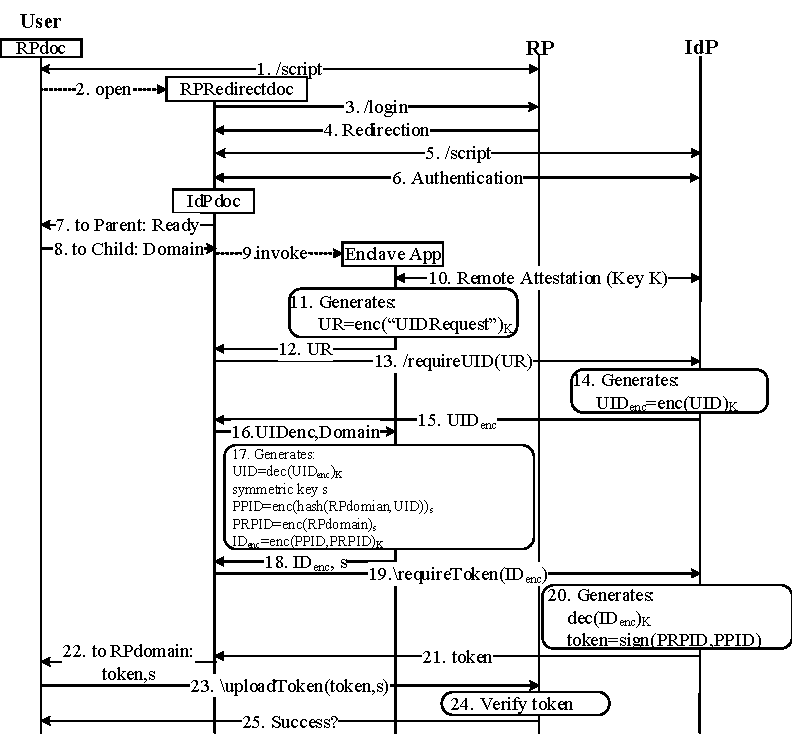
\includegraphics[width=0.8\linewidth]{fig/sgx-sso.pdf}
  \caption{The protocol flow of UP-SSO.}
  \vspace{-5mm}
  \label{fig:UP-SSO}
\end{figure*}
%The UP-SSO is compatible with OIDC, besides that the IdP service is separated into user part and server part. 
%The user agent (i.e., user-side IdP service) would obtain the UID from server part service, transform UID into the PPID, and encrypt the RPID and PPID with a one-time symmetric key to avoid IdP server digging out the RP's identity. As the enclave application is protected by SGX, it must not conduct any malicious behaviour. 
%The server-side IdP service takes the responsibility of authenticating the user, retrieving the UID for each user, and issuing the identity token (i.e., the identity proof) consisted the privacy-preserving RP and user identifier.

In this section, we will provide the detailed protocol.

%\subsection{UP-SSO procedures}
\subsection{Initialization}
%\vspace{1mm}\noindent\textbf{RP registration.} 
At the very beginning, RP needs to register its domain, RP name and other essential attributes at IdP, and obtains a signed Cert.  Thus, the  IdP can only provide the service to the qualified RP by checking the ownership of a Cert inside the enclave application.

%\vspace{1mm}\noindent\textbf{Preparation work of user .} 
Moreover, user should install the enclave application on her device before the visit targeting an RP. 

\subsection{Login Process}
Following, we provide the detailed process of each authentication flow shown as Figure~\ref{fig:UP-SSO}.
%The procedures of UP-SSO are depicted in detail in Figure~\ref{fig:UP-SSO}. 
It can be split into three phases, scripts downloading, PPIDs generation and identity proof issuing. To be noticed that, all the communication flows among user, RP server and IdP server are protected by TLS.

\vspace{0.5mm}\noindent\textbf{Scripts downloading.} This phase is for the user’s browser to download the scripts from the RP and IdP. The SSO process is started with the user's visit to an RP at her browser, and the browser downloads the RP script (step 1). Then the RP script opens a new window targeting RP login endpoint (step 2, 3). After that the user is redirected to the IdP server (step 4). Finally, the user retrieves the IdP script (step 5).

It must be noticed that, the user cannot visit IdP at step 2,3 directly. While the script in origin A opens a new window with origin B, the HTTP request to B's server will carry the key-value $Referer: A$ in the header. Thus, the RP's domain is exposed to IdP. 
% The scripts work as part of the user agent role.
\begin{comment}
\item[1]The SSO process is started with the user's visit to an RP at her browser, and the browser downloads the RP script. 
%The script is used to conduct the behaviour defined by RP on user side.
\item[2]The RP script opens a new window. 
\item[3]The newly opened window visits RP login endpoint.
\item[4]The user is redirected to the IdP server from RP.% login endpoint.
\item[5]The user retrieves the IdP script, which is used to deal with the interaction with other entities.% IdP server, RP script and enclave application.
\end{comment}
%It must be noticed that, the user cannot visit IdP at step 2,3 directly. While the script in origin A opens a new window with origin B, the HTTP request to B's server will carry the key-value $Referer: A$. Thus, the RP's domain is exposed.% to IdP. 
%With HTML5, a special attribute for links in HTML was introduced, that the $ref="noreferrer"$ can be used to make $Referer$ header be suppressed. However, when such a link is used to open a new window, the new window does not have a handle on the opening window (opener) anymore. The handle is necessary for UP-SSO to transmit messages between RP and IdP scripts. 
%So the redirection is adopted to avoid the HTTP header $Referer$. %and make the handle of the opening window available. 


\vspace{0.5mm}\noindent\textbf{PPIDs Generation.} In this phase, IdP script invokes the enclave application to generate the PPID. 
At first, the IdP authenticates the user (step 6). 
After that, IdP script informs RP window (step 7), and RP script sends its Cert to IdP script (step 8).  
Then IdP script asks for user's consent to visit targeting RP, and it invokes the enclave application (step 9). 
The enclave application conducts remote attestation at its initialized execution, and negotiates a symmetric key $K$ with IdP server (step 10).
Following the enclave application generates the UID request by encrypting request information with $K$ (step 11). 
The request is sent to IdP script (step 12) and transmitted to IdP server (step 13). 
IdP encrypts $UID$ with $K$ (step 14), and transmits it to enclave application through IdP script (step 15, 16).  
While receiving the encrypted $UID$, the enclave application derives the $UID$, verifies the Cert and achieves RP's domain from it, generates the symmetric key $S$, encrypts the RP's domain as the  $PPID_{RP}$, encrypts the hash of RP's domain and UID as the $PPID_U$, and encrypts $PPID_{RP}$ and $PPID_U$ with $K$ (step 17). 
Finally the encrypted IDs and $S$ are sent to IdP script (step 18). 

The $PPID_U$ must be the encrypted hash of RP's domain and UID, instead of the plain digest. It avoids the IdP to find out multiple logins targeting the same RP or not, as the hash of same RP's domain would be always the same. 

%Moreover, there are some types of parameters required in OIDC protocol to be carried in the SSO request, such as $response\_type$ and $scope$. In this paper, we would not mention these attributes, and only focus on the necessary parameters. 
\begin{comment}
\item[6]At first, the IdP authenticates the user.
\item[7]After the IdP script is downloaded, it sends the ready signal to its opener (i.e., the RP window).
\item[8]RP script sends the RP's Cert back to IdP script. 
\item[9] The IdP script shows RP name to user to make sure user would not visit malicious RP, and then it invokes the enclave application.
\item[10]The enclave application conducts remote attestation at its initialized execution. After the remote attestation, enclave application and IdP server share a symmetric key $K$.
\item[11]The enclave application generates the UID request (i.e., $UR$) by encrypting request information with $K$.
\item[12]$UR$ is sent to IdP script.
\item[13]Then the user starts the UID request to IdP.
\item[14]IdP encrypts $UID$ with $K$.
\item[15]IdP script receives encrypted $UID$ from IdP.
\item[16]IdP script transmits encrypted $UID$ and RP's domain to enclave application.
\item[17]The enclave application derives the $UID$ with $K$, verifies the Cert, achieves RP's domain from Cert, generates the symmetric key $s$, encrypts the RP's domain with key $s$ as the transformed RP ID (i.e., $PRPID$), encrypts the hash of RP's domain and UID as the $PPID$, and encrypts $PRPID$ and $PPID$ with $K$.
\item[18]Enclave application sends the encrypted IDs and $s$ to IdP script. 
\end{comment} 
%The PPID must be the encrypted hash of RP's domain and UID, instead of the plain digest. It avoids the IdP to find out multiple logins targeting the same RP or not, as the hash of same RP's domain would be always the same. 

%Moreover, there are some types of parameters required in OIDC protocol to be carried in the SSO request, such as $response\_type$ and $scope$. In this paper, we would not mention these attributes, and only focus on the necessary parameters. 

\vspace{0.5mm}\noindent\textbf{Identity proof issuing.} In this phase, IdP issues an identity proof containing the encrypted $PPID_{RP}$ and $PPID_U$. And the RP verifies the token.
At the beginning user sends the encrypted $PPID_{RP}$ and $PPID_U$ to IdP for identity proof (step 19). 
Then the IdP server derives the $PPID_{RP}$ and $PPID_U$, signs the $Token$ consisted of $PPID_{RP}$ and $PPID_U$ as the identity proof (step 20), and sends it to IdP script (step 21). 
The IdP script then sends the $oken$ and $s$ to the origin RP's $Domain$ through $postMessage$ (step 22), and  RP script uploads them to RP server (step 23). 
The RP server verifies the signature with IdP's public key, compares the $PPID_{RP}$ carried with identity proof with self-generated one, and derives the constant user account from $PPID_U$ (step 24). 
%generates the $PRPID$ with its domain and key $s$, and compared it with the one carried by $token$. If the two $PRPID$s are equaled, RP decrypts the user's account from $PPID$, and finds out the related user information in its database (step 24). 
At the end, RP returns the login result back to user (step 25).


\begin{comment}
\item[19]User sends the encrypted $PRPID$ and $PPID$ to IdP for identity proof.
\item[20]The IdP server derives the $PRPID$ and $PPID$, signs the $token$ consisted of $PRPID$ and $PPID$ as the identity proof.
\item[21]IdP sends identity token to enclave application.
\item[22]The IdP script then sends the $token$ and $s$ to the origin RP's $Domain$ through $postMessage$.
\item[23]The RP script uploads the $token$ and key $s$ to RP server.
\item[24]The RP server firstly verifies the signature with IdP's public key, then generates the $PRPID$ with its domain and key $s$, and compared it with the one carried by $token$. If the two $PRPID$s are equaled, RP decrypts the user's account from $PPID$, and finds out the related user information in its database.
\item[25]RP returns the login result back to user.
\end{comment} 

%The origin required in step 22 
%is essential for secure identity token transmitting.
%It 
%guarantees that only the script running in the RP window can receive the $Token$, that avoids the man-in-the-middle attack.


\section{Security Analysis}
\label{sec:analysis}
This section presents the analysis of security and privacy. 

\subsection{Security of UP-SSO}
We summarize the basic requirements of SSO systems based on existing theoretical analyses~\cite{ArmandoCCCT08,FettKS16, FettKS17} and practical attacks~\cite{SomorovskyMSKJ12,WangCW12,ArmandoCCCPS13,WangZLG16,MainkaMS16,MainkaMSW17,YangLCZ18}. These requirements enable an SSO system to provide secure authentication services for RPs.
\begin{itemize}
%\item
%\textbf{User identification.} When a user logs in to an RP multiple times,
 %the RP extracts the identical user identifier from identity proofs.
%    to provide personalized services for this user.

\item
\textbf{RP designation.} The designated RP is specified in identity proof,
    so that this identity proof is  only accepted by this RP.


\item
\textbf{Integrity and confidentiality.}
 Only the IdP can generate identity proofs,
and the identity proof with any modification would not be accepted.
Meanwhile, identity proof is only transmitted to the user and the designated RP.
\end{itemize}

%Although UP-SSO follows the main rules of OIDC, that RP redirects user to IdP, and IdP authenticates the user and returns an identity token back to RP. It also breaks OIDC's mechanisms satisfying the requirements of secure SSO. For example, in OIDC system, to guarantee the confidentiality of identity token, an identity token is transmitted to RP based on the HTTP redirection (i.e., 302 redirection) mechanism, and IdP guarantees the receiver's address belongs to honest RP (verifying \emph{redirect\_uri}). However, in UP-SSO, IdP does not learn the RP's identity, so that it needs to be proved that UP-SSO provides the secure mechanism to guarantee the confidentiality of identity token.

Following, we would describe the security mechanisms provided in UP-SSO system. 

%\vspace{1mm}\noindent\textbf{User identification.}
%UP-SSO does satisfy the requirement as it provides the PPID, from which the RP can derive a constant user account (i.e., the hash of PR domain and UID).%, similarly as it in OIDC system. 


\vspace{1mm}\noindent\textbf{RP designation.} 
%The idea of RP designation is that, IdP issues an identity token for user $Alice$ to visit RP $A$. Once $A$ receives this token, it cannot use the token to visit another RP $B$ as user $Alice$.
Different from identity proof in OIDC system, the proof issued by UP-SSO IdP contains the encrypted RP ID instead of plain one. 
We consider an adversary can get an identity proof
, while the domain may belong to a malicious RP ($PPID_{RP}$ is the encrypted domain, and $PPID_U$ is the encrypted hash of the domain and user's $UID$, while the key is generated by enclave application).
% including $\\PRPID=enc(\mathtt{Malicious Domain})_{key}$ and $\\PPID=enc(hash(\mathtt{Malicious Domain}, UID))_{key}$.
There is no chance to find key $S'$ satisfying that, the honest RP can derive its domain from $PPID_{RP}$, and derive valid user account from $PPID_U$ with the same $S'$, as the user account must equals to the hash of honest RP's domain and honest user's $UID$.
%To be noticed that, the valid user account must equals to the hash of honest RP's domain and honest user's $UID$.
%\newline $dec(PRPID)_{key'} \equiv \mathtt{Honest Domain}$ and  $\\ dec(PPID)_{key'}  \equiv  hash(\mathtt{Honest Domain}, UID)$.


\vspace{1mm}\noindent\textbf{Integrity of identity proof.}
%Although UP-SSO system offers the same identity token as it in OIDC system, 
An adversary may temper the identity proof by offering malicious key at step 22 in Figure~\ref{fig:UP-SSO}. 
We consider  only the IdP server and enclave application are honest. 
An adversary can get an identity proof, 
while the $PPID_{RP}$ and $PPID_U$ are generated with malicious user's $UID$ and any registered RP's domain.
%while the $UID$ must belong to the malicious user, and the domain used for generating $PPID_{RP}$ and $PPID_U$ can be any registered RP domain.
There is no chance an adversary can get a key $S'$ and the domain satisfying that, 
the honest RP can derive its domain from $PPID_{RP}$, and derive the valid user account from $PPID_U$ with the same $S'$. 


\begin{comment}
including 
\newline $PRPID=enc(\mathtt{Any Domain})_{key}$ and 
\newline $PPID=enc(hash(\mathtt{Any Domain}, \mathtt{Malicious UID}))_{key}$. 
%The $Domain$ is controlled by adversary and can be assigned as any value. 
\newline The $Malicious UID$ must belong to the adversary, while the $\mathtt{Any Domain}$ can be any registered RP domain.
There is no chance an adversary can get $key'$  satisfying that, 
\newline $dec(PRPID)_{key'} \equiv \mathtt{Honest Domain}$ and  
\newline $dec(PPID)_{key'} \equiv  hash(\mathtt{Honest RPDomain}, \mathtt{Honest UID})$.
\end{comment}

Moreover, 
%unlike IdP in OIDC system retrieves the PPID from its database, IdP in UP-SSO system needs to receive the PPID from user client. Therefore, 
an adversary may try to lead IdP to issue a token with malicious PPID to break the integrity indirectly.  PPID is generated based on $Domain$ and $UID$, however, the domain is guaranteed by the $Cert$ and $UID$ is protected by the Key $K$. Thus the generation of $PPID_U$ cannot be undermined. Moreover, the $PPID_U$ is protected by $K$ during the transmission, so that it cannot be modified. Therefore, the integrity of identity proof is guaranteed. 
%Here we review Figure~\ref{fig:UP-SSO}. 
\begin{comment}
\item An adversary may attempt to temper the $PPID$ while it is transmitted between enclave application and IdP server. However, $PPID$ is encrypted (step 17) and the key is only known to enclave application and IdP server (key exchange at step 10).
\item The adversary may also try to undermine the generation of $PPID$. 
The $PPID$ is generated based on $RPDomain$ and $UID$ (step 17). According to the description in RP designation, the $RPDomain$ must belong to the target RP. The $UID$ is retrieved according to authentication result at step 6, and encrypted.
\item The adversary may also try to steal an honest user's encrypted $PPID$ and $UID$, and set them in step 16 or step 19. However, in an honest user's device, the IdP script and enclave application are honest, so that they do not send encrypted $PPID$ and $UID$ to any malicious party. Moreover, we consider honest user's device is secure, so that the adversary cannot steal $PPID$ and $UID$ in the manners, such as intercepting communications in user's device.
\end{comment}


\vspace{1mm}\noindent\textbf{Confidentiality of identity proof.}
Confidentiality of identity proof requires that the identity proof must be transmitted to RP correctly without being exposed to adversaries.
%As IdP in UP-SSO system does not learn the target RP's identity, it cannot sends the identity token to RP through an HTTP 302 redirection, which is widely used in SSO systems, such as OIDC. 

To guarantee the identity proof is securely transmitted, $postMessage$ restricted with an origin is adopted in UP-SSO system. That is, while the IdP script receives an identity proof from IdP server, it would invoke the $postMessage$ function provided by browser. And the target's origin is set as the value $RPDomain$ used in generating $PPID_{RP}$ and $PPID_U$. Browser guarantees that only the script belongs to the set origin can receive this identity proof.

%Even an adversary can work as a malicious script in user's browser and conduct malicious behaviour, such as man-in-the-middle attack, it cannot steal user's identity token. That is, while an adversary succeeds in tempering the RP's $Domain$ (at step 8 in Figure~\ref{fig:UP-SSO}), according to proof of RP designation, the identity token would not be accepted by an honest RP. Otherwise, while an adversary does not temper $Domain$, it cannot receive the identity token due to $postMessage$ mechanism.



\subsection{Privacy of UP-SSO}
According to Section~\ref{sec:design}, we can find that a curious IdP can only obtain the $PPID_{RP}$ related to the RP's identity. The $PPID_{RP}$ is the transformed RP domain, which is encrypted with a one-time key. Therefore, the IdP cannot know the real RP's identity or link multiple logins on the same RP. So the IdP-based identity tracing is not possible in UP-SSO system. 

Similarly, the RP can only obtain the $PPID_U$ from IdP. A malicious RP cannot derive the real user's UID from the $hash(Domain, UID)$. Thus, the collusive RPs are also unable to link the same user based on UID. Although the malicious RP can control the RP's $Domain$ to lead the IdP generate incorrect $PPID_U$, it still fails to accomplish the attack. Because due to the proof of confidentiality of identity proof, once the RP's $Domain$ is not consist with the RP's origin, the RP script would be unable to receive the identity proof. Therefore, the attack is not available. 

%However, the attack based on user's cookie is not considered in this paper. That is, the cookie of user may be exploited by malicious RPs to link a user at different RPs. For example, a user may visit multiple RPs at the same time. The malicious RPs may redirect the user to each other through the hidden iframe, carrying the $PPID$. This attack is also available in other user authentication systems besides of SSO system. Moreover, it can be easily detected through multiple methods, such as checking the iframe in the script, observing redirection flow through browser network tool, and detecting the redirection based on the browser extension.



























\begin{comment}
Our formal analysis of XXX is based on the Dolev-Yao style web model~\cite{SPRESSO}, which has been widely used in formal analysis of SSO protocol, e.g., OAuth 2.0~\cite{FettKS16} and OIDC ~\cite{FettKS17}.
To make the description cleaner, we foucus on our communications among XXX entities, and assume DNS and HTTPS are secure, which has already been anaylzed in~\cite{SPRESSO}.


\subsection{The Web Model}

The main entities in the model are $atomic\ processes$, which represent the essential nodes in the web systems, such as browsers, web servers and attackers. The atomic processes communicate with each other through the $events$ containing the receiver atomic process's address (e.g., IP), the sender atomic process process's address and the transmitted $messages$. Moreover, there are also dependent $scripting\ processes$ which runs on the client-side environment relying on the browsers such as JavaScript. The scripting provides the server defined function to the browser.  The web system mainly consists of the set of atomic processes and scripting processes. The operation of a system is described as that the system converts its states via step of runs. The state of web system is called $configuraton$ which consists of all the states of the atomic processes in the system and all the event can be accepted by the processes.

Here, we list the definitions of these notations as follows. 


\vspace{1mm}\noindent\textbf{Message } is defined as formal terms without variables (called ground terms). The messages in the model is considered containing constants (such as ASCII strings and nonce), sequence symbols (such as n-ary sequences $\langle \rangle$, $\langle . \rangle$, $\langle . ,. \rangle$ etc.) and further function symbols (such as encryption/decryption and digital signatures). For example, an HTTP request is a common message in the web model, containing a type $\mathtt{HTTPReq}$, a nonce $n$, a method  $\mathtt{GET}$ or $\mathtt{POST}$,  a domain , a path, URL parameters, request headers, and the body  in the sequence symbol formate. Here is an example for an HTTP GET request for the domain  $\mathtt{exa.com/path?para=1}$ with the headers and body empty.
\begin{equation*}
    m:=\langle\mathtt{HTTPReq},n,\mathtt{GET},exa.com,/path,\langle \langle para, 1\rangle \rangle ,\langle \rangle,\langle \rangle \rangle
\end{equation*}

\vspace{1mm}\noindent\textbf{Event } is the basic communication elements in the model.  An event is the term in the formate $\langle a, f, m \rangle$. In an $event$, the $f$ is the sender's address, the $a$ represents the address receiver, and $m$ is the message transmitted. 

\vspace{1mm}\noindent\textbf{Atomic Process}.  An $atomic\ Dolev-Yao (DY)\ process$ is can be displayed as the tuple $p=$ $(I^p, Z^p, R^p,s_0^p )$, which stands for the single node in the web model, such as the server and browser. $I^p$ includes the addresses owned by this process. $Z^p$ is the set of states that this process is probably in. $R^p$ is the set of relations between the pairs $\langle s, e \rangle$ and $\langle s', e' \rangle$ where $s, s' \in Z^p$.
That is, once a process is in the sate $s$ and receives the event $e$, it would jump into the state $s'$ and wait for the event $e'$.
%is the relation where inputting a state $s \in Z^p$ and an event $e$ and outputting a new state $s'$ and event $e'$, and $s_0 \in Z^p$ is the initial state of the process. 
%It's worth noting that for one process in a state only a finite set of events can be accepted by the process as the state and event are defined as the input of $R^p$.

\noindent\textbf{Browser Process.}
In XXX, we assume that the browsers are honest, therefore, we only need to analyze how the browsers interactive with the scripts. 
The browser model mainly includes the windows and documents.
\begin{itemize}
\item \noindent\textbf{Window}. The window \myss{w} represents the  the concrete browser window in the system, which is identified by a \myss{nonce}. A window contains a set of $\mathtt{documents}$ including the current document and cached documents. 
\item \noindent\textbf{Document}. The document is the HTML content in a window, which is identified by the document \myss{nonce}. It includes the scripting process downloaded from server.
\end{itemize}


\vspace{1mm}\noindent\textbf{Scripting Process}. The web model also contains the scripting process representing the client-side script loaded by browser such as JavaScript code. However, the $scripting\ process$ must rely on an $atom\ process$ such as browser and provide the relation $R$ witch is called by this $atomic\ process$. 

\vspace{1mm}\noindent\textbf{Equational Theory } is defined as usual in Dolev-Yao models,  but introduces the symbol $\equiv$ representing the congruence relation on terms. For instance,  $dec(enc(m,$ $ k),\ k)$ $\equiv$ $m$, where $k$ is the symmetric key.

\vspace{1mm}\noindent\textbf{Web System. }
The web system is consisted of a set of processes (including atomic processes and scripting processes). The web system can be described as the tuple ($\mathcal{W}$, $\mathcal{S}$, $\mathtt{script}$, $E^0$). $\mathcal{W}$ is consisted of the atomic processes, including honest processes and malicious processes. $\mathcal{S}$ is the set of scripting processes including honest scripts and malicious scripts. $\mathtt{script}$ is the set of concrete script code. And $E^0$ includes all the events that could be accepted by the processes in $\mathcal{W}$. 

\vspace{1mm}\noindent\textbf{Configuration}. 
In the web system, there is the set of states of all processes in $\mathcal{W}$ at one point in time, denoted as $S$. 
And all the $event$s can be accepted by the processes at this point consist the set $E$.
A $configuration$ of the system is defined as the tuple ($S, E, N$) where $N$ is the mentioned sequence of unused nonces. 

\vspace{1mm}\noindent\textbf{Run Step}. A run step is the process, that a web system changes its configuration ($S, E, N$) into ($S', E', N'$) after accepting an event $e \in E$. 

\subsection{Model Of XXX}
The XXX model is a web system which is defined as 
\begin{equation*}
    \mathcal{XWS} = (\mathcal{W}, \mathcal{S}, \mathtt{script}, E^0),
\end{equation*}

$\mathcal{W}$ is the finite set of atom processes in XXX system including a single IdP server process, multiple honest RP server processes, the browser processes, the enclave application processes and the attacker processes. We assume that all the honest RPs are implemented following the same rule so that the process are considered consistent besides of the addresses they listen to. The browsers controlled by user are considered honest. That is, the browser controlled by attackers can behave as  an independent atomic process. The enclave applications are always honest.

$\mathcal{S}$ is the finite set of scripting processes consists of $script\_rp$, $script\_idp$ and $script\_attacker$. The $script\_rp$ and $script\_idp$ are downloaded from honest RP and IdP processes and the $script\_attacker$ is downloaded from attacker process considered existing in all browser processes. 

\subsection{Security of XXX}
In this section, we prove the security of XXX. Here, we give the theorem to be proved. 
\begin{theorem}
Let $\mathcal{XWS}$ be the XXX web system, then $\mathcal{EWS}$ is secure.
\label{the:secure}
\end{theorem} 

The XXX is considered secure  {\sl iff} the adversary cannot log in to an honest RP under another honest user's account. Based on the model of XXX, described in Appendix~\ref{sec:appendix}, only when the RP accepts an valid identity proof and retrieves the PPID same as the honest user's from adversary, the attack is successful. Therefore, we can get the definition.

\begin{definition}
Let $\mathcal{XWS}$ be an XXX web system, $\mathcal{XWS}$ is secure \emph{iff} the adversary cannot obtain a valid identity proof, whose encrypted PPID could be decrypted into the honest user's PPID.
\label{def:secure}
\end{definition}

To prove XXX system is secure, we only need to guarantee that it satisfies the requirements described in definition~\ref{def:secure}. 
The adversary may try to retrieve a valid identity proof in following ways: (1) forging the valid identity proof itself; (2) leading the honest RP treat adversary's identity proof as the honest user's one; (3) stealing a valid token from an honest entity in the system. 
Therefore, definition~\ref{def:secure} can be further classified into the following lemmas. 

\begin{lemma}
The adversary cannot forge the valid identity proof.
\label{lem:forge}
\end{lemma}

\begin{proof}
It can be easily proved that, while an RP receives the identity proof, it verifies the signature with the public key of the IdP. Only the IdP knows the corresponding private key, so that the adversary cannot forge the valid identity proof itself.
\end{proof}

\begin{lemma}
The RP would not retrieve an honest user's PPID from the adversary's identity proof.
\label{lem:trickRP}
\end{lemma}

\begin{proof}
The adversary cannot obtain the identity proof issued for other honest user from XXX system, which is to be proved in lemma~\ref{lem:steal}. We consider in the SSO process, only the IdP server and enclave application are honest. An adversary can get a identity proof including $\mathtt{PRPID}=encrypt(\mathtt{Domain})$ and $\mathtt{PRPID}=encrypt(hash(\mathtt{Domain}, \mathtt{uid}))$. The $\mathtt{Domain}$ is controlled by adversary and can be assigned as any value. The $\mathtt{uid}$ must belong to the adversary. There is no chance that an adversary can get a key, making the attack available. Because the key must satisfy that, $decrypt(\mathtt{PRPID}, key) \equiv honest\ RPDomain$ and  $decrypt(\mathtt{PPID}, key) \equiv hash(honest\ RPDomain, honest\ uid)$, which is not possible.   
\end{proof}


\begin{lemma}
The adversary cannot steal an identity proof from any entities in the system.
\label{lem:steal}
\end{lemma}

\begin{proof}
We first give an outline of the proof. (1) For IdP, it only sends the identity proof to its enclave application. (2) For enclave application, it only returns the token back to whom invoked it with the uid token. And it can be proved that only the honest user can own the uid token beside of enclave application and IdP server. (3) The IdP script only transmits the token to the script in the origin $\mathtt{RPDomain}$. As the identity proof includes the $\mathtt{PRPID}$, the identity proof would be only sent to the origin that the token is issued for. (4) The RP script only sends the identity proof to its server. (5) RP sever would not send identity proof to any parties.
The detailed proof is described as follows. 

The identity proof sent by IdP is shown in line 44, Algorithm~\ref{alg1}, as the response of path described in line 38, Algorithm~\ref{alg1}. We consider that IdP only accepts the enclave application's request to path $\mathtt{requireUID}$ and $\mathtt{requireToken}$. Therefore, the identity proof would only be sent to the enclave application.

We can see that the identity proof is sent by enclave application shown in line 25, Algorithm~\ref{alg5} to the entity defined in line 2, ~\ref{alg5}. The receiver of identity proof is the one invoking it with a uid token (line 4, Algorithm~\ref{alg5}). And the uid is exchanged with this uid token (line 9, 14, Algorithm~\ref{alg5}). 
Then we prove that the only the honest user can own the uid token. Based on line 11-16 and line 22-28, Algorithm, we can see that IdP only sends the uid token to the authenticated user. It can be observed that the IdP script receives the uid token in line 34, Algorithm~\ref{alg3} and only sends it to enclave application in line 35, Algorithm~\ref{alg3}. Therefore, an adversary cannot obtain a user's uid token, so that it cannot retrieve the identity proof from the enclave application.

The IdP script only sends the identity proof by postMessage shown at line 43, Algorithm~\ref{alg3}. The target is the opener of this window and restricted by the origin $mathtt{RPDomain}$. $\mathtt{RPDomain}$ is defined at line 25, Algorithm~\ref{alg3} and never rewrote. Due to the scriptstate, in Algorithm~\ref{alg3} the $\mathtt{RPDomain}$s used at line 35 (used for identity proof generation) and line 43 (restricting the receiver) must be consistent with the one at line 25. Therefore, IdP would not send the identity proof to any adversaries. 

The model Algorithm~\ref{alg4} shows RP script receives the identity proof at line 21 and send it out at line 25, while the receiver is defined at line 23. The receiver address is assigned during initiation at line 4 and never modified. It is downloaded with the script and considered honest. Therefore, the RP script would not send the identity proof to adversary.

Based on the model shown as Algorithm~\ref{alg2}, we can find that RP server would not send identity proof to other parties. Therefore, the adversary cannot steal the identity proof from RP server.
\end{proof}

It is proved that XXX system satisfies the requirements raised in definition~\ref{def:secure}. Therefore, Theorem~\ref{the:secure} is proved.



\subsection{Privacy of UP-SSO}
Based on the process shown in Section~\ref{sec:design}, we can find that a curious IdP can only obtain the $PRPID$ related with the RP's identity. The $PRPID$ is the transformed RP domain, which is encrypted with an one-time key. Therefore, the IdP cannot know the real RP's identity or link multiple logins on the same RP. So the IdP-based identity tracing is not possible in UP-SSO system. 

Similarly, the RP can only obtains the $PPID$ from IdP. An malicious RP cannot derive the real user's UID from the $hash(RPDomain, UID)$. The collusive RPs are also unable to link the same user because of the same reason. Although the malicious RP can control the $RPDomain$ to lead the IdP generate incorrect $PPID$, it still fails to accomplish the attack. Because due to the proof of confidentiality, once the $RPDomain$ is not consist with the RP's origin, the RP script would be unable to receive the identity proof. Therefore, the attack is not available. 

However, the attack based on user's cookie is not considered in this paper. That is, the cookie of user may be exploited by malicious RPs to link a user at different RPs. For example, a user may visit multiple RPs at the same time. The malicious RPs may redirect the user to each other through the hidden iframe, carrying the $PPID$. This attack is also available in other user authentication systems beside of SSO system. Moreover, it can be easily detected through multiple methods, such as checking the iframe in the script, observing redirection flow through browser network tool, and detecting the redirection based on the browser extension.

\end{comment}



\section{Implementation and Evaluation}
\label{sec:implementation}
We have implemented  a prototype of UP-SSO.
%, containing an IdP server, an RP server and the user client. 
In this section, we describe the details of implementation and compare it with the open-source OIDC project to show its practical value.
\subsection{Implementation}
We adopt SHA-256 for digest generation, RSA-2048 for signature generation, and 128-bit AES/GCM algorithm for symmetrical encryption. 


IdP and RP servers are implemented based on Spring Boot, a popular web framework. 
We use the open-source auth0/java-jwt library to generate and verify the identity proof. 
The cryptographic computations of servers are implemented using API provided by JDK. 
Native messaging~\cite{NativeMessaging} (enables communication between chrome extension and native application) and chrome extension are  adopted to enable the JavaScript code to invoke the native application installed on user's device. 
%Native messaging offers the channel for chrome extension to communicate with native application. And chrome extension can communicate with the JavaScript code in the browser. 
%Many popular browsers have already supported native messaging, such as chrome and firefox. 
Enclave application is built based on Intel enclave SDK,
which offers the APIs for cryptographic computations.%, under hardware-level protection. 

\subsection{Evaluation}
\noindent\textbf{Environment.}
In the evaluation, we deploy the RP and IdP servers on the device with Intel i7-8700 CPU and 32GB RAM memory, running Windows 10 x64 system. The browser is Chrome v90.0.4430.212, deployed on the same device.   



\vspace{1mm}\noindent\textbf{Result.}
We have run SSO process on our prototype system 100 times, and the average time is 154 ms (from user visiting an RP to RP returning the authentication result). As the remote attestation overhead is only counted once the enclave application is initiated, the overhead is not included in the result (about xx ms). For comparison, we run MITREid Connect, a popular open-source OpenID Connect project. The time cost of  MITREid Connect is 113 ms. The overhead is modest.
\section{Related Works}
\label{sec:relatedwork}
%\subsection{Security and Privacy of SSO system}
%Recently, SSO systems have been the essential infrastructure of internet service. Various SSO protocols, such as OAuth, OIDC and SAML are  widely adopted by Google, Facebook and other companies. There are also troubles about the security and privacy that are introduced with the SSO systems. 

\noindent\textbf{Security analysis of SSO systems.} Various attackers were found accessing the honest user's account at RP by multiple methods. 
Some attackers exploit the vulnerabilities of user's platforms to steal  identity proof (or cookie)~\cite{WangCW12,ArmandoCCCPS13}.
Some other attackers temper the identity proof to impersonate an honest user, such as XSW~\cite{SomorovskyMSKJ12}, RP's incomplete verification~\cite{WangCW12,WangZLG16,MainkaMSW17}, and IdP spoofing~\cite{MainkaMS16,MainkaMSW17}. 
Some IdP services did not bind the identity proof with a corresponding RP (or the honest RP did not verify the binding), so that malicious RP can leverage the received identity proof to access to another RP~\cite{WangZLG16,MainkaMS16,MainkaMSW17}. 
The formal analysis is also used to guarantee the security of SSO protocols~\cite{FettKS16,FettKS17}.
%Moreover, automatical tools, such as SSOScan~\cite{ZhouE14}, OAuthTester~\cite{YangLLZH16} and S3KVetter~\cite{YangLCZ18}, are also designed to detect vulnerabilities in SSO systems.

%Besides the analysis of the implemented SSO systems, the formal analysis is also used to guarantee the security of SSO protocols. Fett et al.~\cite{FettKS16, FettKS17} analyze the OAuth 2.0 and OIDC protocols based on the expressive Dolev-Yao style model~\cite{FettKS14}. The vulnerabilities found in these analyses enable the adversary steals the identity token form SSO systems. The analysis also shows that OAuth 2.0 and OIDC are secure once these two vulnerabilities are prevented. 

\vspace{1mm}\noindent\textbf{Privacy-preserving SSO systems.} NIST~\cite{NIST2017draft} suggests that the SSO should prevent user's trace from being tracked by both RP and IdP. 
%The pairwise user identifier (e.g., PPID) is used in some SSO protocols, such as SAML~\cite{SAML} and OIDC~\cite{OpenIDConnect}. 
Some protocols simply hide the RP's identity from IdP, such as SPRESSO~\cite{SPRESSO} (using encrypted RP identifier) and BrowserID~\cite{BrowserID} (RP identifier is added by user). However,  they are not defensive to RP-based identity linkage, and cannot integrate PPID. 
%Moreover, an analysis on Persona found IdP-based login tracing could still succeed~\cite{FettKS14, BrowserID}.
There is also another method that prevents both IdP and RP from knowing user's trace based on zero-knowledge algorithm, such as EL PASSO~\cite{ZhangKSZR21} and UnlimitID~\cite{IsaakidisHD16}. However, this type of solution requires user should remember a secret representing her identity, which is not convenient for login on multiple devices.

%Anonymous SSO schemes enable the users to access a service (i.e. RP) with permission from a verifier (i.e., IdP) without revealing their identities.
%The anonymous SSO systems are designed based on multiple methods. For example, various cryptographic primitives, such as group signature, zero-knowledge proof, etc., were used to design anonymous SSO schemes~\cite{WangWS13,HanCSTW18}. 
%The anonymous SSO schemes allow a user to obtain an unidentified token anonymously, and access RP's service with this token. However, the RP cannot classify a user's multiple logins, as the user is completely anonymous in this system. Therefore, they are not available in current personalized internet service.

%\subsection{Intel SGX}
%Intel SGX and remote attestation have been already used in many fields, particularly in authentication and building a trusted environment. 

\vspace{1mm}\noindent\textbf{Authentication systems built based on Intel SGX.} Intel SGX has been used in enhancing the security and privacy of authentication systems. Rafael et al.~\cite{CondeMW18} offer the credential protection approach based on SGX, which prevents an adversary from stealing a user's credential at server side. P2A~\cite{SongWLOWL20} is proposed to protect user's privacy. It enables a user to generate an identity proof locally while the registration, update, freeze/thaw, and deletion of identities are managed in a blockchain. Therefore, a user can visit a service without exposing her real identity. 

\begin{comment}
Remote attestation is wisely adopted on building the trusted environment. Jaehwan et al.~\cite{AhnLK20} propose a method
of building a safe smart home environment for IoT by pre-blocking devices based on remote attestation. 
Uzair et al.~\cite{JavaidAS20} establish the trust between IoT devices based on the blockchain and remote attestation, while the blockchain offers a secure framework for device registration. Moreover, there is work on how to conduct the remote attestation without an assigned key or secure memory (required in Intel SGX). Ilia et al.~\cite{LebedevHD18} propose the design of an attested execution processor based on RISC-V Rocket chip architecture. It does not 
require secure non-volatile memory, nor a private key explicitly assigned by the manufacturer.
\end{comment}
\section{Conclusion}
\label{sec:conclusion}
We propose UP-SSO,
%enhancing the User Privacy of SSO by Integrating PPID and SGX.
%UP-SSO is
the extended PPID-based SSO system with comprehensive protections against both the IdP-based login tracing and the RP-based identity linkage.
To prevent the IdP from knowing a user's login trace in an SSO system, we split the IdP service into two parts, and shift the PPID generation from server to user-controlled environment.
This part of service runs on the user's device protected by the Intel SGX. The integrity is guaranteed through the remote attestation, even the malicious user cannot control the user-side service.
%The server-side service takes the responsibility of authenticating users, storing the private key, issuing the identity token and etc.
%The other part generates the PPID based on the user identifier retrieved by server-part service, and transforms PPID and RP's identifier into one-time encrypted ID to prevent both IdP-based user tracing and RP-based identity linkage.
We systemically analyze the UP-SSO protocol and guarantee its security.
We have implemented the prototype of UP-SSO system, and the performance evaluation on the prototype demonstrates the  overhead is modest.


\bibliographystyle{splncs04}
\bibliography{ref}

%\newpage
\appendix
\section{Appendix: Web Model}
%\begin{appendices}
\subsection{Message Format}
Here we provide the details of the format of the messages we use to construct the ExtraF model.

\vspace{1mm}\noindent\textbf{HTTP Messages}.
An HTTP request message is the term of the form
\vspace{-3mm}
\begin{equation*}
\langle \mathtt{HTTPReq}, nonce, method, host, path, parameters, headers, body\rangle
\end{equation*}

An HTTP response message is the term of the form
\vspace{-2mm}
\begin{equation*}
    \myangle{\mathtt{HTTPResp}, nonce, status, headers, body}
\end{equation*}
 The details are defined as follows:
 \begin{itemize}
 \item \myss{\mathtt{HTTPReq}} and \myss{\mathtt{HTTPResp}} denote the types of messages.
 \item \myss{nonce} is a random number that maps the response to the corresponding request.
 \item \myss{method} is the HTTP methods, such as \myss{\mathtt{GET}} and \myss{\mathtt{POST}}.
 \item \myss{host} is the constant string domain of visited server.
 \item \myss{path} is the constant string representing the concrete resource of the server.
 \item \myss{parameters} contains the parameters carried by the url as the form \\ \myss{\myangle{\myangle{name, value}, \myangle{name, value}, \dotsc}}, for example, the \myss{parameters} in the url \myss{http://www.example.com?type=confirm}  is \myss{\myangle{\myangle{type, confirm}}}.
 \item \myss{headers} is the header content of each HTTP messages as the form \\ \myss{\myangle{\myangle{name, value}, \myangle{name, value}, \dotsc}}, such as \\ \myss{\langle\myangle{Referer, http://www.example.com},} \myss{\myangle{Cookies, c}\rangle}.
 \item \myss{body} is the body content carried by HTTP \myss{\mathtt{POST}} request or HTTP response in the form \myss{\myangle{\myangle{name, value}, \myangle{name, value}, \dotsc}}.
  \item \myss{status} is the HTTP status code defined by HTTP standard.
 \end{itemize}

\vspace{1mm}\noindent\textbf{URL}.
URL is a term \myss{\myangle{\mathtt{URL}, protocol,host,path,parameters}}, where \myss{\mathtt{URL}} is the type, \myss{protocol} is chosen in \myss{\{\mathtt{S}}, \myss{\mathtt{P}\}} as \myss{\mathtt{S}} stands for HTTPS and \myss{\mathtt{P}} stands for HTTP. The \myss{host, path}, and \myss{parameters} are the same as in HTTP messages.

\vspace{1mm}\noindent\textbf{Origin}.
An Origin is a term \myss{\myangle{host, protocol}} that stands for the specific domain used by the HTTP CORS policy, where \myss{host} and \myss{protocol} are the same as in URL.

\vspace{1mm}\noindent\textbf{POSTMESSAGE}.
PostMessage is used in the browser for transmitting messages between scripts from different origins. We define the postMessage as the form \myss{\myangle{\mathtt{POSTMESSAGE}, target, Content, Origin}}, where \myss{\mathtt{POSTMESSAGE}} is the type, \myss{target} is the constant nonce which stands for the receiver, \myss{Content} is the message transmitted and \myss{Origin} restricts the receiver's origin.

\vspace{1mm}\noindent\textbf{XMLHTTPREQUEST}.
XMLHTTPRequest is the HTTP message transmitted  by scripts in the browser. That is, the XMLHTTPRequest is converted from the HTTP message by the browser. The XMLHTTPRequest in the form \myss{\myangle{\mathtt{XMLHTTPREQUEST}, URL, methods, Body, nonce}} can be converted into HTTP request message by the browser, and \myss{\myangle{\mathtt{XMLHTTPREQUEST}, Body, nonce}}  is converted from HTTP response message.

\vspace{1mm}\noindent\textbf{ENCLAVEMESSAGE}.
EnclaveMessage is the message transmitted between Script Process and Enclave Application. It is defined as the term \\ \myss{\myangle{\mathtt{ENCLAVEMESSAGE}, Content}}.


\noindent\textbf{Data Operation}.
The data used in ExtraF are defined in the following forms:
\begin{itemize}
\item \textbf{Standardized Data} is the data in the fixed format, for instance, the HTTP request is the standardized data in the form \myss{\langle\mathtt{HTTPReq}}, \myss{nonce}, \myss{method}, \myss{host}, \myss{path}, \myss{parameters}, \myss{headers}, \myss{body\rangle}.  We assume there is an HTTP request \myss{r :=}  \myss{\langle\mathtt{HTTPReq}},  \myss{n},  \myss{\mathtt{GET}},  \myss{example.com},  \myss{/path},  \myss{\myangle{}},  \myss{\myangle{}},  \myss{\myangle{}\rangle}, here we define the operation on the $r$. That is, the elements in $r$ can be accessed in the form \myss{r.name}, such that \myss{r.method \equiv \mathtt{GET}},  \myss{r.path \equiv /path} and \myss{r.body \equiv \myangle{}}.
\item \textbf{Dictionary Data} is the data in the form \myss{\myangle{\myangle{name, value}, \myangle{name, value}, \dotsc}}, for instance the \myss{body} in HTTP request is dictionary data. We assume there is a \myss{body := \myangle{\myangle{username, alice}, \myangle{password, 123}}}, here we define the operation on the $body$. That is, we can access the elements in \myss{body} in the form \myss{body[name]}, such that \myss{body[username] \equiv alice} and \myss{body[password] \equiv 123}.
%We can also add the new attributes to the dictionary, for example after we set \myss{body[age] := 18}, the \myss{body} are changed into\myss{ \myangle{\myangle{username, alice}, \myangle{password, 123}, \myangle{age, 18}}}.
\end{itemize}

\subsection{Browser Model}
In UPPRESSO, we assume that the browsers are honest, therefore, we only need to analyze how the browsers interactive with the scripts. 
We first introduce the windows and documents of the browser model.

\vspace{1mm}
\noindent\textbf{Window}. A window \myss{w} is a term of the form \myss{w = \myangle{nonce, documents, opener}}, representing the  the concrete browser window in the system. The \myss{nonce} is the window reference to identify each windows. The \myss{documents} is the set of documents (defined below) including the current document and cached documents (for example, the documents can be viewed via the ``forward" and ``back" buttons in the browser). The \myss{opener} represents the window in which this window is created, for instance, while a user clicks the href in document \myss{d} and it creates a new window \myss{w}, there is \myss{w.opener \equiv d.nonce}.

\vspace{1mm}
\noindent\textbf{Document}. A document \myss{d} is a term of the form
\begin{multline*}
\langle nonce, location, referrer, script, scriptstate, \\
 scriptinputs, subwindows, active \rangle 
\end{multline*}
where document is the HTML content in the window.  The \myss{nonce} locates the document. \myss{Location} is the URL where the document is loaded. \myss{Referrer} is same as the Referer header defined in HTTP standard. The \myss{script} is the scripting process downloaded from each servers. \myss{scriptstate} is define by the script, different in each scripts. The \myss{scriptinputs} is the message transmitted into the scripting process. The \myss{subwindows} is the set of \myss{nonce} of document's created windows. \myss{active} represents whether this document is active or not.

A scripting process is the dependent process relying on the browser, which can be considered as a relation \myss{R} mapping a message input and a message output. And finally the browser will conduct the command in the output message. Here we give the description of the form of input and output.
\begin{itemize}
\setlength\itemsep{-2pt}
\item \textbf{Scripting Message Input. } The input is the term in the form
\begin{multline*}
\langle tree, docnonce, scriptstate, stateinputs,cookies,\\
localStorage, sessionStorage, ids, secret \rangle
\end{multline*}
\item \textbf{Scripting Message Output. }The output is the term in the form
\begin{equation*}
\langle scriptstate, cookies, localStorage,sessionStorage, command \rangle
\end{equation*}
\end{itemize}
The \myss{tree} is the relations of the opened windows and documents, which are visible to this script. \myss{Docnonce} is the document nonce. The  \myss{Scriptstate} is a term of the form defined by each script. \myss{Scriptinputs} is the message transmitted to script. However, the \myss{scriptinputs} is defined as standardized forms, for example, postMessage is one of the forms of \myss{scriptinputs}. \myss{Cookies} is the set of cookies that belong to the document's origin. \myss{LocalStorage} is the storage space for browser and \myss{sessionStorage} is the space for each HTTP sessions.  \myss{Ids} is the set of user IDs while \myss{secret} is the password to corresponding user ID. The \myss{command} is the operation which is to be conducted by the browser. Here we only introduce the form of commands used in XXX system. We have defined the postMessage and XMLHTTPRequest (for HTTP request) message which are the \myss{commands}. Moreover, a term in the form \myss{\myangle{\mathtt{IFRAME}, URL, WindowNonce}} asks the browser to create this document's subwindow and it visits the server with the URL.

\subsection{XXX Model}

\noindent\textbf{IdP server}.

\begin{breakablealgorithm}
  \caption{$R^i$}
  \label{alg1}
  \begin{algorithmic}[1]
  \Require{\myss{\myangle{a, f, m}, s}}
  \mystate{\myss{s':=s}}
  \mystate{\myss{n, method, path, parameters, headers, body} \textbf{such that}}\\
  \ \ \myss{\myangle{\mathtt{HTTPReq},n,method,path,parameters,headers,body} \equiv m}\\
  \ \ \textbf{if} \myss{possible}; \textbf{otherwise} stop \myss{\myangle{}, s'}
  \myif{path \equiv /script}
  \mystate{\myss{m':=\myangle{\mathtt{HTTPResp},n,200, \myangle{}, \mathtt{IdPScript}}}}
  \mystop{f, a, m'}
  
  \myelse{path \equiv /login}
  \mystate{\myss{cookie := headers[Cookie]}}
  \mystate{\myss{session := s'.sessions[cookie]}}
  \mystate{\myss{username:=body[username]}}
  \mystate{\myss{password:=body[password]}}
  \myif{password \not\equiv \mathtt{SecretOfID}(username)}
  \mystate{\myss{m' :=\myangle{\mathtt{HTTPResp},n,200,\myangle{},\mathtt{LoginFailure}}}}
  \mystop{f,a,m'}
  \EndIf
  \mystate{\myss{session[uid] := \mathtt{UIDOfUser}(username)}}
  \mystate{\myss{m' :=\myangle{\mathtt{HTTPResp},n,200,\myangle{},\mathtt{LoginSucess}}}}
  \mystop{f,a,m'}
  
  \myelse{path \equiv /requireUIDToken}
  \mystate{\myss{cookie := headers[Cookie]}}
  \mystate{\myss{session := s'.sessions[cookie]}}
  \mystate{\myss{uid := session[uid]}}
  \myif{uid \equiv \mathtt{null}}
  \mystate{\myss{m' := \myangle{\mathtt{HTTPResp},n,200,\myangle{},\mathtt{UnLogged}}}}
  \mystop{f,a,m'}
  \EndIf
  \mystate{\myss{token := \mathtt{GenerateToken}()}}
  \mystate{\myss{s'.Tokens := s'.Tokens + ^{\myangle{}}\myangle{uid, token}}}
  \mystate{\myss{m' := \myangle{\mathtt{HTTPResp},n,200,\myangle{},\myangle{\mathtt{Token}, token}}}}
  \mystop{f,a,m'}
  
  \myelse{path \equiv /requireUID}
  \mystate{\myss{UIDToken := body[UIDToken]}}
  \mystate{\myss{uid := \mathtt{FindUIDByToken(UIDToken)}}}
  \myif{uid \equiv null}
  \mystate{\myss{m' := \myangle{\mathtt{HTTPResp}, n, 200, \myangle{}, \mathtt{TokenError}}}}
  \mystop{f,a,m'}
  \EndIf
  \mystate{\myss{m' := \myangle{\mathtt{HTTPResp}, n, 200, \myangle{}, \myangle{\mathtt{UID}, uid}}}}
  \mystop{f,a,m'}
  
  \myelse{path \equiv /requireToken}
  \mystate{\myss{PRPID := body[PRPID]}}
  \mystate{\myss{PPID := body[PPID]}}
  \mystate{\myss{Content := \myangle{PRPID,PPID}}}
  \mystate{\myss{token := Content+Sign(Content,s'.SignKey)}}
  \mystate{\myss{m' := \myangle{\mathtt{HTTPResp}, n, 200, \myangle{}, \myangle{\mathtt{Token},token}}}}
  \mystop{f,a,m'}
  \EndIf
  \mystop{}
  \end{algorithmic}
\end{breakablealgorithm}

\noindent\textbf{RP server}.

\begin{breakablealgorithm}
  \caption{$R^r$}
  \label{alg2}
  \begin{algorithmic}[1]
  \Require {\myss{\myangle{a, f, m}, s}}
  \mystate{\myss{s':=s}}
  \mystate{\myss{n, method, path, parameters, headers, body} \textbf{such that}}\\
  \ \ \myss{\myangle{\mathtt{HTTPReq},n,method,path,parameters,headers,body} \equiv m}\\
  \ \ \textbf{if} \myss{possible}; \textbf{otherwise} stop \myss{\myangle{}, s'}
  \myif{path \equiv /script}
\mystate{\myss{m':=\myangle{\mathtt{HTTPResp},n,200, \myangle{}, \mathtt{RPScript}}}}
  \mystop{f, a, m'}
  
  \myelse{path \equiv /uploadToken}
  \mystate{\myss{cookie := headers[Cookie]}}
  \mystate{\myss{session := s'.sessions[cookie]}}
  \mystate{\myss{token := body[Token]}}
  \mystate{\myss{key := body[Key]}}
  \myif{\mathtt{CheckSig}(Token.Content, Token.Sig, s'.IdP.PubKey)}
  \mystate{\myss{PRPID := \mathtt{Encrypt}(s'.RPDomain,key)}}  
  \myif{PRPID \equiv token.Content.PRPID}
  \mystate{\myss{PPID := token.Content.PPID}}
  \myif{PPID \not \in \mathtt{ListOfUser}()}
  \mystate{\myss{\mathtt{RegisterUser}(PPID)}}
  \EndIf
  \mystate{\myss{session[user] := PPID}}
  \mystate{\myss{m' := \myangle{\mathtt{HTTPResp}, n, 200, \myangle{}, \mathtt{LoginSuccess}}}}
  \EndIf
  \EndIf
  \mystate{\myss{m' := \myangle{\mathtt{HTTPResp}, n, 200, \myangle{}, \mathtt{Fail}}}}
  \mystop{f, a, m'}
  \EndIf
  \mystop{}
  \end{algorithmic}
\end{breakablealgorithm}


\noindent\textbf{IdP script}.

\begin{breakablealgorithm}
  \caption{$script\_idp$}
  \label{alg3}
  \begin{algorithmic}[1]
  \Require{\myss{\langle tree, docnonce, scriptstate, scriptinputs, cookies, localStorage,}}
  \Statex {\myss{ sessionStorage, ids, secret \rangle}}  
  \mystate{\myss{ s' := scriptstate}}
  \mystate{\myss{command := \myangle{}}}
  \mystate{\myss{target := \mathtt{PARENTWINDOW}(tree,docnonce)}}
  \mystate{\myss{IdPDomain := s'.IdPDomain}}
  \SWITCH{\myss{s'.q}}
    \CASE{\myss{startLogin}}
    \mystate{\myss{username \in ids}}
    \mystate{\myss{Url := \myangle{\mathtt{URL}, \mathtt{S}, IdPDomain, /login, \myangle{}}}}
    \mystate{\myss{s'.refXHR :=  \mathtt{Random}()}}
    \mystate{\myss{command : = \langle \mathtt{XMLHTTPREQUEST}, Url, \mathtt{POST},}}  
    \Statex \myss{\ \ \ \ \ \ \ \ \ \ \myangle{\myangle{username, username}, \myangle{password, secret}}, s'.refXHR \rangle}
    \mystate{\myss{s'.q := expectLoginResult}}
    \ENDCASE
    
    \CASE{expectLoginResult}
      \mystate{\myss{pattern := \myangle{\mathtt{XMLHTTPREQUEST},Body,s'.refXHR}}}
      \mystate{\myss{input := \mathtt{CHOOSEINPUT}(scriptinputs,pattern) }}
      \myif{input \not\equiv \mathtt{null}}
      \myif{input.Body \not\equiv \mathtt{LoginSuccess}}
      \mystate{\myss{\textbf{stop}\ \myangle{}}}
      \EndIf
      \mystate{\myss{command := \myangle{\mathtt{POSTMESSAGE}, target, \mathtt{Ready}, \mathtt{null}}}}
      \mystate{\myss{s'.q := expectRPDomain}}
      \EndIf
      \ENDCASE
    
    \CASE{\myss{expectRPDomain}}
      \mystate{\myss{pattern := \myangle{\mathtt{POSTMESSAGE}, *, Content, *}}}
      \mystate{\myss{input := \mathtt{CHOOSEINPUT}(scriptinputs,pattern)}}
      \myif{input \not\equiv \mathtt{null}}
      \mystate{\myss{RPDomain := input.Content[RPDomain]}}
      \mystate{\myss{s'.Parameters[RPDomain] := RPDomain}}
      \mystate{\myss{Url := \myangle{\mathtt{URL}, \mathtt{S}, IdPDomain, /requireUIDToken,\myangle{} }}}
      \mystate{\myss{s'.refXHR :=  \mathtt{Random}()}}
      \mystate{\myss{command : = \langle\mathtt{XMLHTTPREQUEST}, Url, \mathtt{GET}, s'.refXHR\rangle}}
      \mystate{\myss{s'.q := expectUIDToken}}
       \EndIf
      \ENDCASE
      
    \CASE{expectUIDToken}
      \mystate{\myss{pattern := \myangle{\mathtt{XMLHTTPREQUEST},Body,s'.refXHR}}}
      \mystate{\myss{input := \mathtt{CHOOSEINPUT}(scriptinputs,pattern) }}
      \myif{input \not\equiv \mathtt{null}}
      \mystate{\myss{token := input.Body[UIDToken]}}
      \mystate{\myss{command := \myangle{\mathtt{ENCLAVEMESSAGE}, \myangle{\mathtt{UIDToken}, token}}}}
      \mystate{\myss{s'.q := expectIdentityToken}}
      \EndIf
      \ENDCASE
    
    \CASE{expectIdentityToken}
      \mystate{\myss{pattern := \myangle{\mathtt{ENCLAVEMESSAGE},Content}}}
      \mystate{\myss{input := \mathtt{CHOOSEINPUT}(scriptinputs,pattern) }}
      \myif{input \not\equiv \mathtt{null}}
      \mystate{\myss{token:=input.Content[Token]}}
      \mystate{\myss{key:=input.Content[Key]}}
      \mystate{\myss{command := \langle\mathtt{POSTMESSAGE}, target, \langle\myangle{\mathtt{IdentityToken}, token},}}
      \Statex \myss{\ \ \ \ \ \ \ \ \ \ \ \ \ \ \myangle{\mathtt{Key},key} \rangle ,\mathtt{s'.Parameters[RPDomain]}\rangle}
      \mystate{\myss{s'.q := stop}}
      \EndIf
      \ENDCASE 
  \ENDSWITCH
\mystate{\myss{\textbf{stop}\ \myangle{s',cookies,localStorage,sessionStorage,command}}}
    \end{algorithmic}
\end{breakablealgorithm}


\noindent\textbf{RP script}.

\begin{breakablealgorithm}
  \caption{$script\_rp$}
  \label{alg4}
  \begin{algorithmic}[1]
\Require {\myss{\langle tree, docnonce, scriptstate, scriptinputs, cookies, localStorage,}} 
\Statex \myss{sessionStorage, ids, secret\rangle}
\mystate{\myss{ s' := scriptstate}}
  \mystate{\myss{command := \myangle{}}}
  \mystate{\myss{IdPWindow := \mathtt{SUBWINDOW}(tree,docnonce).nonce}}
  \mystate{\myss{RPDomain := s'.RPDomain}}
  \SWITCH{\myss{s'.q}}
    \CASE{\myss{start}}
    \mystate{\myss{Url := \myangle{\mathtt{URL}, \mathtt{S}, RPDomain, /login, \myangle{}}}}
    \mystate{\myss{command := \myangle{\mathtt{IFRAME}, Url, \_SELF}}}
    \mystate{\myss{s'.q := expectReady}}
    \ENDCASE
    \CASE{\myss{expectReady}}
    \mystate{\myss{pattern := \myangle{\mathtt{POSTMESSAGE}, *, Content, *}}}
      \mystate{\myss{input := \mathtt{CHOOSEINPUT}(scriptinputs,pattern)}}
      \myif{input \not\equiv \mathtt{null} \land input.Content \equiv \mathtt{Ready}}
      \mystate{\myss{Content := \myangle{\mathtt{\mathtt{RPDomain}},RPDomain}}}
      \mystate{\myss{command := \myangle{\mathtt{POSTMESSAGE}, target, Content, \mathtt{null}}}}
      \mystate{\myss{s'.q := expectToken}}
      \EndIf
      \ENDCASE
      \CASE{\myss{expectToken}}
      \mystate{\myss{pattern := \myangle{\mathtt{POSTMESSAGE}, *, Content, *}}}
      \mystate{\myss{input := \mathtt{CHOOSEINPUT}(scriptinputs,pattern) }}
      \myif{input \not\equiv \mathtt{null}}
      \mystate{\myss{token := input.Content[Token]}}
      \mystate{\myss{key := input.Content[Token]}}
      \mystate{\myss{Url := \myangle{\mathtt{URL}, \mathtt{S}, RPDomain, /uploadToken, \myangle{}}}}
      \mystate{\myss{s'.refXHR :=  \mathtt{Random}()}}
      \mystate{\myss{command : = \langle \mathtt{XMLHTTPREQUEST}, Url, \mathtt{POST},}}
      \Statex \myss{\ \ \ \ \ \ \ \ \ \ \ \ \ \  \myangle{\myangle{\mathtt{Token}, token},\myangle{\mathtt{Key},key}}, s'.refXHR\rangle}
      \mystate{\myss{s'.q := stop}}
      \EndIf
      \ENDCASE
     \ENDSWITCH
\end{algorithmic}
\end{breakablealgorithm}



\noindent\textbf{Enclave application}.

\begin{breakablealgorithm}
  \caption{$R^e$}
  \label{alg2}
  \begin{algorithmic}[1]
  \Require {\myss{\myangle{a, f, m}, s}}
  \mystate{\myss{s':=s}}
  \mystate{\myss{\mathtt{InvokeFrom}:=f}}
  \myif{m.type \equiv \mathtt{ENCLAVEMESSAGE}}
  \mystate{\myss{token := m.Content[Token]}}
  \mystate{\myss{RPDomain := m.Content[RPDomain]}}
  \mystate{\myss{s'.Parameters[RPDomain]:=RPDomain}}
  \myif{token \not \equiv null}
  \mystate{\myss{n_1 = \mathtt{RANDOM}() }}
  \mystate{\myss{m' := \langle \mathtt{HTTPReq}, n_1, \mathtt{POST}, s'.IdP.Host, s'.IdP.UIDToken, }}
  \Statex \myss{\ \ \ \ \ \ \ \ \ \  \myangle{\myangle{\mathtt{UIDToken}, token}}\rangle}
  \mystop{s'.IdP.Address, \mathtt{\_SELF}, m'}
  \EndIf
  \EndIf
  \mystate{\myss{n, headers, body} \textbf{such that}} \myss{\myangle{\mathtt{HTTPResp},n, 200, headers,body} \equiv m}\\
  \ \ \textbf{if} \myss{possible}; \textbf{otherwise} stop \myss{\myangle{}, s'}
  \myif{n \equiv n_1}
  \mystate{\myss{uid :=body[UID]}}
	\myif{uid \not \equiv null}
	\mystate{\myss{key := \mathtt{GenerateKey()}}}	
	\mystate{\myss{PRPID := \mathtt{Encrypt}(s'.Parameters[RPDomain],key)}}
	\mystate{\myss{ PPID:=\mathtt{Encrypt}(\mathtt{Hash}(s'.Parameters[RPDomain],uid),key)}}
	\mystate{\myss{n_2 = \mathtt{RANDOM}() }}
	\mystate{\myss{m' := \langle \mathtt{HTTPReq}, n_2, \mathtt{POST}, s'.IdP.Host, s'.IdP.IdentityToken, }}
  \Statex \myss{\ \ \ \ \ \ \ \ \ \  \myangle{\myangle{\mathtt{PRPID}, PRPID},\myangle{\mathtt{PPID}, PPID}}\rangle}
  \mystop{s'.IdP.Address, \mathtt{\_SELF},  m'}
 \EndIf
 
 \myelse{n \equiv n_2}
 \mystate{\myss{token := body[Token]}}
 \mystate{\myss{m':=\myangle{\mathtt{ENCLAVEMESSAGE}, \myangle{\myangle{\mathtt{Token},token},\myangle{\mathtt{Key},key}}}}}
  \mystop{\mathtt{InvokeFrom}, \mathtt{\_SELF}, m'}
  \EndIf
  \mystop{}
  \end{algorithmic}
\end{breakablealgorithm}


\end{document}
